\documentclass[12pt,a4paper]{article}

\usepackage{amsmath,amssymb,amsthm}
\usepackage{mathtools}
\usepackage{ytableau}
\usepackage{tikz}
\usepackage{enumitem}
\usepackage[margin=2.5cm]{geometry}
\usepackage{hyperref}
\usepackage{booktabs}

% Theorem environments
\newtheorem{theorem}{Theorem}[section]
\newtheorem{proposition}[theorem]{Proposition}
\newtheorem{lemma}[theorem]{Lemma}
\newtheorem{corollary}[theorem]{Corollary}
\theoremstyle{definition}
\newtheorem{definition}[theorem]{Definition}
\newtheorem{example}[theorem]{Example}
\theoremstyle{remark}
\newtheorem{remark}[theorem]{Remark}

% Shortcuts
\newcommand{\C}{\mathbb{C}}
\newcommand{\Z}{\mathbb{Z}}
\newcommand{\N}{\mathbb{N}}
\newcommand{\gl}{\mathfrak{gl}}
\newcommand{\fU}{\mathfrak{U}}
\newcommand{\fD}{\mathfrak{D}}
\newcommand{\fL}{\mathfrak{L}}
\newcommand{\End}{\operatorname{End}}
\newcommand{\Hom}{\operatorname{Hom}}
\newcommand{\Ind}{\operatorname{Ind}}
\newcommand{\Res}{\operatorname{Res}}
\newcommand{\SYT}{\operatorname{SYT}}
\newcommand{\SSYT}{\operatorname{SSYT}}
\newcommand{\shape}{\operatorname{shape}}
\newcommand{\Rep}{\mathcal{R}\text{ep}}
\newcommand{\Vect}{\mathcal{V}\!ect}

\title{The Representation Theory of Local Rules}
\author{Notes}
\date{}

\begin{document}
\maketitle

\begin{abstract}
We explain the representation-theoretic content of Fomin's local rules
for growth diagrams, at increasing levels of generality. At the most
basic level, local rules encode the multiplicity-free branching rule
for the symmetric groups. At the next level, they provide a bijective
realisation of the Mackey formula for induction and restriction, which
is equivalently the normal ordering relation in the Heisenberg
algebra. The consistency of local rules across a growth diagram is the
Yang--Baxter equation. In the cylindric setting, the higher-order
local rules that transform bijections across adjacent profiles encode
the action of the degenerate affine Hecke algebra, and the cylindric
growth diagram is the combinatorial avatar of the Drinfeld functor to
Yangian modules.
\end{abstract}

\tableofcontents

%% ====================================================================
\section{Setup and notation}
\label{sec:setup}
%% ====================================================================

We work over a field $k$ of characteristic zero. Partitions are
denoted $\lambda, \mu, \nu, \ldots$ and written in weakly decreasing
order $\lambda = (\lambda_1 \geqslant \lambda_2 \geqslant \cdots)$.
We write $\lambda \vdash n$ for $|\lambda| = n$ and
$\ell(\lambda)$ for the number of parts.

For a partition $\lambda$, define
\begin{align*}
  U(\lambda) &= \{\,\nu : \nu/\lambda \text{ is a horizontal strip}\,\}
    \quad \text{(partitions obtained by adding a horizontal strip)}, \\
  D(\lambda) &= \{\,\mu : \lambda/\mu \text{ is a horizontal strip}\,\}
    \quad \text{(partitions obtained by removing a horizontal strip)}.
\end{align*}
In the single-box case, $U(\lambda)$ consists of partitions obtained
by adding one box and $D(\lambda)$ those obtained by removing one box.

We write $S^\lambda$ for the Specht module (irreducible representation
of $S_n$, where $\lambda \vdash n$) and $W^\lambda$ for the Weyl
module (irreducible polynomial representation of $\mathrm{GL}_N$ of
highest weight $\lambda$).

%% ====================================================================
\section{Layer 1: Local rules as branching rules}
\label{sec:branching}
%% ====================================================================

\subsection{The multiplicity-free branching rule}

The restriction of an irreducible $S_n$-module to $S_{n-1}$ is
multiplicity-free:
\begin{equation}\label{eq:branching}
  S^\lambda\big|_{S_{n-1}}
  \;=\; \bigoplus_{\mu} S^\mu,
\end{equation}
where $\mu$ ranges over all partitions obtained from $\lambda$ by
removing a single box. This multiplicity-freeness is the essential
structural fact that makes local rules possible: at each step of a
growth diagram, there is a \emph{unique} box being added or removed,
so the local rule can track it deterministically.

The same statement holds for the general linear groups: the branching
$\mathrm{GL}_N \supset \mathrm{GL}_{N-1}$ gives
\[
  W^\lambda\big|_{\mathrm{GL}_{N-1}}
  = \bigoplus_\mu W^\mu,
\]
where $\mu$ satisfies the interlacing condition
$\lambda_1 \geqslant \mu_1 \geqslant \lambda_2 \geqslant \mu_2
\geqslant \cdots$. This is again multiplicity-free and underlies the
Gel'fand--Tsetlin basis.

\subsection{Fomin's local rule}

A \emph{growth diagram} is a rectangular grid whose vertices are
labelled by partitions, with edges going up and to the right,
such that adjacent partitions along any edge differ by at most one box.
Each unit square has four corner partitions:
\[
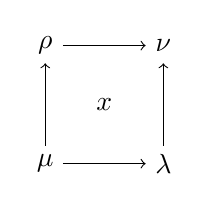
\begin{tikzpicture}[scale=1.5]
  \node at (0,1) {$\rho$};
  \node at (1,1) {$\nu$};
  \node at (0,0) {$\mu$};
  \node at (1,0) {$\lambda$};
  \node at (0.5,0.5) {$x$};
  \draw[->] (0.15,0) -- (0.85,0);
  \draw[->] (0,0.15) -- (0,0.85);
  \draw[->] (1,0.15) -- (1,0.85);
  \draw[->] (0.15,1) -- (0.85,1);
\end{tikzpicture}
\]
Here $x \in \{0,1\}$ is the entry of the input matrix at that cell.
Fomin's \emph{forward local rule} determines $\lambda$ from
$\rho, \mu, \nu$ and $x$:

\begin{enumerate}
\item If $x = 1$ and $\mu = \nu = \rho$: then $\lambda$ is $\rho$
  with one box added to the first row.
\item If $x = 0$ and $\mu = \nu = \rho$: then $\lambda = \rho$.
\item If $x = 0$ and $\mu = \rho \neq \nu$: then $\lambda = \nu$
  (shadow passes vertically).
\item If $x = 0$ and $\nu = \rho \neq \mu$: then $\lambda = \mu$
  (shadow passes horizontally).
\item If $x = 0$ and $\mu, \nu, \rho$ pairwise distinct: then
  $\lambda = \mu \cup \nu$ (two shadows cross).
\item If $x = 0$, $\mu = \nu \neq \rho$, and $\mu$ differs from
  $\rho$ in row $r$: then $\lambda$ is $\mu$ with one box added to
  row $r+1$ (two shadows bounce).
\end{enumerate}

\begin{proposition}
Fomin's local rule applied to a permutation matrix $\sigma \in S_n$
produces a growth diagram whose bottom-right boundary encodes the
insertion tableau $P(\sigma)$ and whose top-right boundary encodes the
recording tableau $Q(\sigma)$ of the Robinson--Schensted correspondence.
\end{proposition}

\subsection{Representation-theoretic content}

Each case of the local rule corresponds to one step of the branching
rule~\eqref{eq:branching}:

\begin{itemize}
\item \textbf{Cases 3--4} (shadow passes through): a restriction path
  from $S^\lambda$ descends through $S^\mu$ on one side and $S^\nu$
  on the other, and these paths are \emph{compatible}---the same box
  is being tracked along both the $S_n$ and $\mathrm{GL}_N$ chains.

\item \textbf{Case 5} (crossing): two independent restriction paths
  pass through the cell without interacting. The box removed to get
  $\mu$ and the box removed to get $\nu$ are in different rows and
  columns, so they commute.

\item \textbf{Case 6} (bouncing): two restriction paths arrive at the
  same partition $\mu = \nu$, having removed the same box from
  $\rho$. The local rule resolves this collision by adding the box
  back in the \emph{next} available position (row $r+1$). This is the
  non-trivial case---it encodes the fact that the branching
  multiplicity is exactly one.
\end{itemize}

The key point: the local rule exists \emph{because} the branching is
multiplicity-free. If $S^\lambda|_{S_{n-1}}$ had multiplicities, there
would be no deterministic way to fill in the fourth corner.

%% ====================================================================
\section{Layer 2: Local rules as the Mackey formula}
\label{sec:mackey}
%% ====================================================================

\subsection{The general local rule}

For semistandard tableaux and the Burge/RSK correspondences, the
single-box local rule generalises to horizontal strips. A
\emph{forward local rule} is a bijection
\begin{equation}\label{eq:forward}
  \fU_{\alpha,\beta}
  \;:\; \bigl(\Z_{\geqslant 0}\,,\; D(\alpha) \cap D(\beta)\bigr)
  \;\xrightarrow{\;\sim\;}\;
  U(\alpha) \cap U(\beta)
\end{equation}
satisfying the \emph{weight condition}: if
$\lambda = \fU_{\alpha,\beta}(m, \mu)$ then
\begin{equation}\label{eq:weight}
  |\lambda| + |\mu| = |\alpha| + |\beta| + m.
\end{equation}
The \emph{reverse local rule} is its inverse:
\begin{equation}\label{eq:reverse}
  \fD_{\alpha,\beta}
  \;:\; U(\alpha) \cap U(\beta)
  \;\xrightarrow{\;\sim\;}\;
  \bigl(\Z_{\geqslant 0}\,,\; D(\alpha) \cap D(\beta)\bigr).
\end{equation}
The integer $m$ is the crucial new ingredient absent from the
single-box case.

\subsection{The Pieri operators}

On the ring of symmetric functions $\Lambda$, define the
\emph{Pieri operator} $\Omega[Xv]$ and its dual $\Omega^*[Xu]$ by
their action on the Schur basis:
\begin{align}
  \Omega[Xv] \cdot s_\mu
  &= \sum_{\substack{\lambda \in U(\mu)}} v^{|\lambda/\mu|}\, s_\lambda,
  \label{eq:pieri-op} \\
  \Omega^*[Xu] \cdot s_\lambda
  &= \sum_{\substack{\mu \in D(\lambda)}} u^{|\lambda/\mu|}\, s_\mu.
  \label{eq:dual-pieri-op}
\end{align}
These operators satisfy the commutation relation
\begin{equation}\label{eq:pieri-comm}
  \Omega^*[Xu]\;\Omega[Xv]
  \;=\; \frac{1}{1 - uv}\;\Omega[Xv]\;\Omega^*[Xu].
\end{equation}

\subsection{The local rule as bijective Mackey formula}

\begin{theorem}\label{thm:local-mackey}
The forward local rule $\fU_{\alpha,\beta}$ provides a bijective proof
of the commutation relation~\eqref{eq:pieri-comm}. Specifically, it
witnesses the identity
\[
  \langle s_\alpha \mid \Omega^*[Xu]\;\Omega[Xv]\; s_\beta \rangle
  \;=\;
  \frac{1}{1-uv}\;
  \langle s_\alpha \mid \Omega[Xv]\;\Omega^*[Xu]\; s_\beta \rangle
\]
as a weighted bijection between the two sides, where the factor
$\frac{1}{1-uv} = \sum_{m \geqslant 0} (uv)^m$ is accounted for by
the integer $m$.
\end{theorem}

Now we interpret this representation-theoretically. The Pieri operator
$\Omega[Xv]$ corresponds to \textbf{induction}: the Pieri rule
$s_\mu \cdot h_k = \sum_\lambda s_\lambda$ (summing over horizontal
strips $\lambda/\mu$ of size $k$) computes
\[
  \Ind_{S_n \times S_k}^{S_{n+k}}\bigl(S^\mu \boxtimes \mathbf{1}_{S_k}\bigr)
  \;=\; \bigoplus_{\lambda/\mu \text{ horiz.\ strip, } |\lambda/\mu|=k} S^\lambda.
\]
The dual operator $\Omega^*[Xu]$ corresponds to \textbf{restriction}
followed by projection onto the trivial representation of the
``removed'' factor.

The commutation relation~\eqref{eq:pieri-comm} therefore says:
\begin{quote}
\emph{``First induce, then restrict'' equals $\frac{1}{1-uv}$ times
``first restrict, then induce.''}
\end{quote}
This is a \textbf{Mackey-type decomposition}. In the classical Mackey
formula, the double cosets $S_{n-j} \backslash S_n / (S_{n-k} \times
S_k)$ control the relationship between induction and restriction.
The integer $m$ in the local rule~\eqref{eq:forward} is precisely the
contribution from the ``identity double coset''---the part where
induction and restriction interact non-trivially.

\begin{remark}
The weight condition~\eqref{eq:weight} has a natural interpretation:
$|\lambda| - |\alpha|$ is the size of the horizontal strip added on
the $\alpha$-side, $|\beta| - |\mu|$ is the size of the strip removed
on the $\beta$-side, and $m$ is the deficit---the number of boxes that
``pass through'' from the removal to the addition without being
accounted for by the strips. It is the Mackey correction term.
\end{remark}

%% ====================================================================
\section{Layer 3: Local rules as normal ordering in the Heisenberg algebra}
\label{sec:heisenberg}
%% ====================================================================

\subsection{The Heisenberg algebra and Fock space}

Consider the Heisenberg algebra $\mathfrak{h}$ generated by operators
$a_n, a_n^\dagger$ ($n \geqslant 1$) satisfying
\[
  [a_m,\, a_n^\dagger] = m\,\delta_{m,n}, \qquad
  [a_m, a_n] = [a_m^\dagger, a_n^\dagger] = 0.
\]
The \emph{Fock space} $\mathcal{F}$ has a basis
$\{|\lambda\rangle : \lambda \text{ a partition}\}$ and carries the
bosonic representation of $\mathfrak{h}$ via
\begin{align*}
  a_n^\dagger |\lambda\rangle
  &= \sum_{\mu:\, \mu/\lambda \text{ is a border strip of size } n}
     (-1)^{\mathrm{ht}(\mu/\lambda)}\, |\mu\rangle, \\
  a_n |\lambda\rangle
  &= \sum_{\nu:\, \lambda/\nu \text{ is a border strip of size } n}
     (-1)^{\mathrm{ht}(\lambda/\nu)}\, |\nu\rangle.
\end{align*}
Under the boson--fermion correspondence, the ring of symmetric
functions $\Lambda$ is identified with $\mathcal{F}$, with
$s_\lambda \leftrightarrow |\lambda\rangle$.

\subsection{Vertex operators and commutation}

The Pieri operators of Section~\ref{sec:mackey} are (exponential)
vertex operators in this language. Writing
\begin{align*}
  U(v) &= \Omega[Xv] = \exp\Bigl(\sum_{n \geqslant 1}
    \frac{v^n}{n}\, a_n^\dagger\Bigr)
    \quad \text{(creation/induction)}, \\
  D(u) &= \Omega^*[Xu] = \exp\Bigl(\sum_{n \geqslant 1}
    \frac{u^n}{n}\, a_n\Bigr)
    \quad \text{(annihilation/restriction)},
\end{align*}
the commutation relation~\eqref{eq:pieri-comm} becomes the standard
normal ordering identity for vertex operators:
\begin{equation}\label{eq:normal-ordering}
  D(u)\, U(v) = \frac{1}{1-uv}\, U(v)\, D(u).
\end{equation}

In the simplest case ($u = v = 1$, single-box operators), this reduces
to Fomin's relation
\[
  DU - UD = \mathrm{Id},
\]
which is the Heisenberg commutation relation in its most elementary
form, and the algebraic reason that Young's lattice is a
$1$-differential poset.

\subsection{Local rules as normal ordering}

\begin{theorem}\label{thm:normal-ordering}
Each application of a local rule moves one creation operator past one
annihilation operator, picking up the commutator
$\frac{1}{1-uv}$. The full growth diagram computes the normal ordering
of a product of vertex operators.
\end{theorem}

Concretely: a growth diagram with $m$ columns and $n$ rows starts with
a product $D(u_1) \cdots D(u_m)\, U(v_1) \cdots U(v_n)$ (all
annihilation operators to the left). Filling in the grid by local
rules reorders this into the normal-ordered form
$U(v_1) \cdots U(v_n)\, D(u_1) \cdots D(u_m)$ times a product of
commutator factors $\prod_{i,j} \frac{1}{1-u_i v_j}$.

The partition at grid position $(i,j)$ records the intermediate state
after $i$ annihilation operators have been moved past $j$ creation
operators. The integers $m_{i,j}$ produced by the local rules at
each cell are the exponents in the commutator factors.

\begin{remark}
This explains why RSK ``works'': the Robinson--Schensted--Knuth
correspondence is the combinatorial computation of normal ordering
in the Heisenberg algebra. The insertion tableau $P$ records the result
of the creation operators (the $\mathrm{GL}_N$ side), the recording
tableau $Q$ records the result of the annihilation operators (the
$S_n$ side), and the growth diagram tracks the commutation step by step.
\end{remark}

%% ====================================================================
\section{Layer 4: Growth diagram consistency is the Yang--Baxter equation}
\label{sec:YBE}
%% ====================================================================

\subsection{The consistency condition}

A growth diagram is filled in one cell at a time, applying the local
rule at each step. The fundamental property is:

\begin{proposition}[Consistency]
\label{prop:consistency}
The result of filling a growth diagram is independent of the order in
which cells are processed, provided each cell is processed only after
its left and lower neighbours are known.
\end{proposition}

This is a non-trivial statement. Consider a $2 \times 1$ strip of two
horizontally adjacent cells:
\[
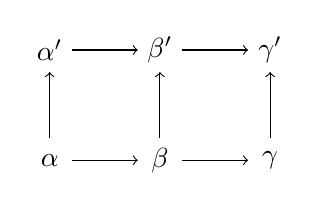
\begin{tikzpicture}[scale=1.4]
  \node at (0,0) {$\alpha$};
  \node at (1,0) {$\beta$};
  \node at (2,0) {$\gamma$};
  \node at (0,1) {$\alpha'$};
  \node at (1,1) {$\beta'$};
  \node at (2,1) {$\gamma'$};
  \draw[->] (0.2,0) -- (0.8,0);
  \draw[->] (1.2,0) -- (1.8,0);
  \draw[->] (0.2,1) -- (0.8,1);
  \draw[->] (1.2,1) -- (1.8,1);
  \draw[->] (0,0.2) -- (0,0.8);
  \draw[->] (1,0.2) -- (1,0.8);
  \draw[->] (2,0.2) -- (2,0.8);
\end{tikzpicture}
\]
Processing left-then-right: first determine $\beta'$ from
$(\alpha', \alpha, \beta)$, then determine $\gamma'$ from
$(\beta', \beta, \gamma)$. This is unambiguous. But for a $2 \times 2$
block:
\[
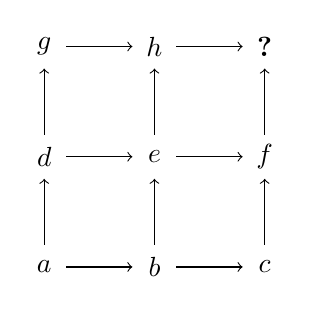
\begin{tikzpicture}[scale=1.4]
  \node at (0,0) {$a$};
  \node at (1,0) {$b$};
  \node at (2,0) {$c$};
  \node at (0,1) {$d$};
  \node at (1,1) {$e$};
  \node at (2,1) {$f$};
  \node at (0,2) {$g$};
  \node at (1,2) {$h$};
  \node at (2,2) {$\boldsymbol{?}$};
  \draw[->] (0.2,0) -- (0.8,0);
  \draw[->] (1.2,0) -- (1.8,0);
  \draw[->] (0.2,1) -- (0.8,1);
  \draw[->] (1.2,1) -- (1.8,1);
  \draw[->] (0.2,2) -- (0.8,2);
  \draw[->] (1.2,2) -- (1.8,2);
  \draw[->] (0,0.2) -- (0,0.8);
  \draw[->] (1,0.2) -- (1,0.8);
  \draw[->] (2,0.2) -- (2,0.8);
  \draw[->] (0,1.2) -- (0,1.8);
  \draw[->] (1,1.2) -- (1,1.8);
  \draw[->] (2,1.2) -- (2,1.8);
\end{tikzpicture}
\]
the cell marked $\boldsymbol{?}$ can be reached by two routes: first
fill the top-left cell $(e)$ then go right to get $f$, then up to get
$\boldsymbol{?}$; or first fill the bottom-right cell $(e)$ then go up
to get $h$, then right to get $\boldsymbol{?}$. Consistency demands
that both routes give the same answer.

\subsection{The Yang--Baxter equation}

This consistency condition is precisely the \textbf{Yang--Baxter
equation} (YBE) in combinatorial form.

In Davydov--Molev's framework~\cite{DM}, the free symmetric monoidal
category $\mathcal{S}$ is generated by one object $X$ and an
involutive Yang--Baxter operator $c : X \otimes X \to X \otimes X$
satisfying
\begin{equation}\label{eq:YBE}
  (c \otimes 1_X)(1_X \otimes c)(c \otimes 1_X)
  = (1_X \otimes c)(c \otimes 1_X)(1_X \otimes c).
\end{equation}
Under the symmetric fiber functor $F_N : \mathcal{S} \to \Vect$ (which
sends $X \mapsto V = k^N$), the operator $c$ becomes the swap map
$\tau : v \otimes w \mapsto w \otimes v$ on $V^{\otimes 2}$.

Now consider the growth diagram as a lattice model. At each vertex,
the local rule acts---it is the combinatorial $R$-matrix. The three
strands in the YBE~\eqref{eq:YBE} correspond to three rows (or
columns) of the growth diagram, and the two sides of the equation
correspond to the two orders of processing a $2 \times 2$ block.

\begin{theorem}\label{thm:local-rule-YBE}
The local rule for growth diagrams satisfies the Yang--Baxter
equation: for any valid boundary data on a $2 \times 2$ block, the
partition at the final corner is independent of the order of
evaluation.
\end{theorem}

\begin{remark}
In the single-box case (Fomin's rules for permutations), the
$R$-matrix is \emph{involutive}: $c^2 = 1$. This corresponds to the
classical case where the symmetric groups $S_n$ are generated by
involutions. In the Hecke algebra case, $c$ satisfies $(c-q)(c+q^{-1})
= 0$ instead, giving a Yang--Baxter operator that is no longer
involutive but satisfies a quadratic relation. The corresponding local
rules are those of van Leeuwen's ``Hecke insertion.''
\end{remark}

%% ====================================================================
\section{Layer 5: Cylindric local rules and the degenerate affine
  Hecke algebra}
\label{sec:cylindric}
%% ====================================================================

We now explain the deepest layer of the dictionary, connecting the
higher-order local rules of~\cite{Langer} for cylindric partitions to
the degenerate affine Hecke algebra $\Lambda_n$ and the Drinfeld
functor of Davydov--Molev~\cite{DM}.

\subsection{The degenerate affine Hecke algebra}

\begin{definition}
The \emph{degenerate affine Hecke algebra} $\Lambda_n$ is the
associative algebra generated by elements
$t_1, \ldots, t_{n-1}$ and $y_1, \ldots, y_n$ subject to:
\begin{align}
  t_i^2 &= 1, \label{eq:daha-inv}\\
  t_i t_{i+1} t_i &= t_{i+1} t_i t_{i+1}, \label{eq:daha-braid}\\
  t_i t_j &= t_j t_i \quad\text{for } |i-j|>1, \label{eq:daha-comm-t}\\
  y_i t_i - t_i y_{i+1} &= 1, \label{eq:daha-yt}\\
  y_i y_j &= y_j y_i, \label{eq:daha-comm-y}\\
  y_j t_i &= t_i y_j \quad\text{for } j \neq i, i{+}1.
    \label{eq:daha-comm-yt}
\end{align}
\end{definition}

As shown in~\cite{DM}, the degenerate affine Hecke algebras form a
multiplicative sequence $\Lambda_* = \{\Lambda_n \mid n \geqslant 0\}$
via the maps $t_i \otimes 1 \mapsto t_i$,
$1 \otimes t_j \mapsto t_{j+m}$, $y_i \otimes 1 \mapsto y_i$,
$1 \otimes y_j \mapsto y_{j+m}$. The associated monoidal category
$\mathcal{L} = \mathcal{C}(\Lambda_*)$ is the \emph{degenerate affine
Hecke category}, a free monoidal category generated by one object $X$,
an endomorphism $x : X \to X$, and an involutive Yang--Baxter operator
$c : X \otimes X \to X \otimes X$ satisfying (in addition to $c^2 = 1$
and the YBE):
\begin{equation}\label{eq:affine-rel}
  (a \otimes b)\, c = c\, (b \otimes a), \qquad a, b \in A = k[y],
\end{equation}
or equivalently $(x \otimes 1)\,c - c\,(1 \otimes x) = 1$.

\subsection{Cylindric partitions and profiles}

A \emph{cylindric partition} of profile $\pi$ is a sequence of
partitions $(\mu^0, \mu^1, \ldots, \mu^T = \mu^0)$ such that
consecutive pairs satisfy interlacing conditions determined by
$\pi$. The profile $\pi$ specifies, at each step $i$, whether
$\mu^{i-1}/\mu^i$ is a horizontal strip ($\pi_i = 0$, a
``descent'') or $\mu^i/\mu^{i-1}$ is a horizontal strip
($\pi_i = 1$, an ``ascent'').

The generating function for cylindric partitions of profile $\pi$
involves an alternating product of Pieri operators
$\Omega[Xv_i]$ and dual Pieri operators $\Omega^*[Xu_j]$, applied
cyclically around the cylinder.

\subsection{The higher-order local rule}

\begin{definition}[\cite{Langer}]
The \emph{higher-order local rule} $\fL_i$ transforms a bijection
for cylindric partitions of profile $\pi$ into a bijection for
the adjacent profile $\pi'$, where $\pi'$ is obtained from $\pi$ by
transposing the $i$-th and $(i{+}1)$-th entries:
\[
  \fL_i : \bigl(\text{bijections for profile } \pi\bigr)
  \;\longrightarrow\;
  \bigl(\text{bijections for profile } \pi'\bigr).
\]
Concretely, given a cylindric partition
$\mathfrak{c} = (\mu^0, \ldots, \mu^T)$ of profile $\pi'$,
the rule $\fL_i$ applies the elementary local rule
$\fU_{\mu^{i-1}, \mu^{i+1}}$ to replace the $i$-th slice:
\[
  \mu^i \;\longmapsto\; \fU_{\mu^{i-1},\, \mu^{i+1}}(m, \mu^i)
  \quad\text{or}\quad
  (m, \mu^i) = \fD_{\mu^{i-1},\, \mu^{i+1}}(\mu^i),
\]
depending on the direction of the profile change.
\end{definition}

\subsection{The representation-theoretic content}

The dictionary between cylindric local rules and the degenerate affine
Hecke algebra is:

\begin{center}
\renewcommand{\arraystretch}{1.5}
\begin{tabular}{@{}lll@{}}
\toprule
\textbf{Cylindric partitions} & \textbf{Degenerate affine Hecke algebra}
  & \textbf{Representation theory} \\
\midrule
Profile $\pi$ & Ordering of $y_i$'s and $t_j$'s
  & Evaluation parameters \\
Adjacent transposition $\pi \to \pi'$
  & Generator $t_i \in \Lambda_n$
  & Swap of adjacent factors \\
Higher-order rule $\fL_i$
  & Action of $t_i$ on modules
  & Elementary intertwiner \\
Evaluation parameter at slice $i$
  & Generator $y_i \in \Lambda_n$
  & Jucys--Murphy element \\
Consistency of $\fL_i \fL_{i+1} \fL_i$
  & Braid relation~\eqref{eq:daha-braid}
  & YBE \\
$\fL_i$ commutes with $y_j$ ($j \neq i, i{+}1$)
  & Relation~\eqref{eq:daha-comm-yt}
  & Locality \\
Profile rotation (cyclic shift)
  & Trace over auxiliary space
  & Cylindric character \\
\bottomrule
\end{tabular}
\end{center}

\begin{theorem}[Informal]\label{thm:drinfeld}
The cylindric growth diagram, viewed as the composition of
higher-order local rules $\fL_i$ that rotate the profile around the
cylinder, is the combinatorial incarnation of the \emph{Drinfeld
functor}
\[
  D_N : \mathcal{L} \to Y(\gl_N)\text{-}\mathrm{Mod}
\]
from Davydov--Molev~\cite{DM}, evaluated on the vector representation
$V \otimes k[y]$.
\end{theorem}

The argument is as follows:

\begin{enumerate}
\item The Drinfeld functor $D_N$ sends the generator $X$ of
  $\mathcal{L}$ to $V \otimes k[y]$, where $V = k^N$. The
  endomorphism $D_N(x)$ is multiplication by $y$ in $k[y]$. The
  Yang--Baxter operator $D_N(c)$ is the involution
  $F_N(c) = \partial + t\tau$, where $\partial$ is the divided
  difference operator
  \[
    \partial f(y_1, y_2) = \frac{f(y_1, y_2) - f(y_2, y_1)}{y_1 - y_2}
  \]
  and $\tau$ is the transposition of variables.

\item On tensor powers, $D_N(X^{\otimes n})$ is a module over the
  Yangian $Y(\gl_N)$. The degenerate affine Hecke algebra $\Lambda_n$
  acts on $D_N(X^{\otimes n}) = (V \otimes k[y])^{\otimes n}
  \simeq V^{\otimes n} \otimes k[y_1, \ldots, y_n]$, with $t_i$
  acting by the divided difference operator on the $i$-th and
  $(i{+}1)$-th variables, and $y_i$ acting by multiplication.

\item A cylindric partition of profile $\pi$ with evaluation
  parameters $v_1, \ldots, v_n$ corresponds to a weight vector in this
  module. The slice sequence
  $(\mu^0, \mu^1, \ldots, \mu^T)$ records the branching path through
  the $\mathrm{GL}_N$ restriction chain, and the profile $\pi$
  specifies the ordering of creation and annihilation operators.

\item The higher-order local rule $\fL_i$ implements the action of
  $t_i$ on this weight vector: it swaps two adjacent slices while
  applying the divided difference correction. The integer $m$ produced
  by the elementary local rule is the divided difference contribution
  $\frac{f(y_i, y_{i+1}) - f(y_{i+1}, y_i)}{y_i - y_{i+1}}$.

\item The full rotation of the profile---composing $\fL_i$'s to cycle
  through all orderings---computes the trace of the product of
  $R$-matrices around the cylinder. This trace is the \emph{transfer
  matrix} of the integrable lattice model, whose eigenvalues are the
  cylindric Schur functions.
\end{enumerate}

\subsection{Borodin's identity as Yangian integrability}

The bijective proof of Borodin's identity in~\cite{Langer} works by
iterating $\fL_i$ to transform a cylindric partition of one profile
into one of another, accumulating integer partitions (the ``inner
partition'' $\gamma$) along the way. The total weight is preserved at
each step by the weight condition~\eqref{eq:weight}.

In the Yangian language, Borodin's identity
\[
  \sum_{\pi} \mathrm{CPP}(\pi;\, q)
  = \prod_{i,j} \frac{1}{1 - x_i y_j} \cdot
    \prod_{i<j} \frac{1}{(1 - x_i x_j)(1 - y_i y_j)}
\]
is a statement about the \textbf{commutativity of transfer matrices}:
the transfer matrices for different spectral parameters commute
because the underlying $R$-matrix satisfies the Yang--Baxter equation.
The product formula on the right-hand side arises from the eigenvalues
of the commuting transfer matrices, computed via the Bethe ansatz or
(in the degenerate case) the Yangian representation theory.

The bijective proof via local rules is the \emph{combinatorial Bethe
ansatz}: each application of $\fL_i$ is one step of diagonalising the
transfer matrix, and the integers $m$ produced at each step are the
Bethe roots.

%% ====================================================================
\section{Summary: the five-layer dictionary}
\label{sec:summary}
%% ====================================================================

\begin{center}
\renewcommand{\arraystretch}{1.6}
\begin{tabular}{@{}p{3.2cm}p{4.5cm}p{5cm}@{}}
\toprule
\textbf{Combinatorics} & \textbf{Representation theory}
  & \textbf{Algebra / Category theory} \\
\midrule
Fomin local rule (single box)
  & Branching $S_n \downarrow S_{n-1}$
  & Restriction functor \\
General local rule $\fU_{\alpha,\beta}$
  & Mackey formula for $\Ind$/$\Res$
  & Commutation of induction and restriction functors \\
Pieri commutation
  & Normal ordering
  & Heisenberg algebra $[a, a^\dagger] = 1$ \\
Growth diagram consistency
  & Yang--Baxter equation
  & $R$-matrix / Yang--Baxter object in $\mathcal{S}$ \\
Higher-order rule $\fL_i$ (cylindric)
  & $t_i$ action on Yangian modules
  & Drinfeld functor $D_N : \mathcal{L} \to Y(\gl_N)$-Mod \\
Cylindric profile rotation
  & Transfer matrix trace
  & Commutativity of Yangian transfer matrices \\
Borodin's identity (bijective proof)
  & Integrability / Bethe ansatz
  & Categorical action of $\mathcal{L}$ \\
\bottomrule
\end{tabular}
\end{center}

\begin{thebibliography}{99}

\bibitem{Borodin}
A.~Borodin,
\emph{Periodic Schur process and cylindric partitions},
Duke Math.\ J.\ \textbf{140} (2007), 391--468.

\bibitem{DM}
A.~Davydov and A.~Molev,
\emph{A categorical approach to classical and quantum Schur--Weyl
duality},
preprint.

\bibitem{Drinfeld}
V.~G.~Drinfeld,
\emph{Degenerate affine Hecke algebras and Yangians},
Funct.\ Anal.\ Appl.\ \textbf{20} (1986), 56--58.

\bibitem{Fomin}
S.~Fomin,
\emph{Schensted algorithms for dual graded graphs},
J.\ Algebraic Combin.\ \textbf{4} (1995), 5--45.

\bibitem{Langer}
R.~Langer,
\emph{Cylindric partitions and Littlewood--Richardson coefficients},
PhD thesis, University of Melbourne, 2012.

\bibitem{Lusztig}
G.~Lusztig,
\emph{Affine Hecke algebras and their graded version},
J.\ Amer.\ Math.\ Soc.\ \textbf{2} (1989), 599--635.

\bibitem{OkounkovVershik}
A.~Okounkov and A.~Vershik,
\emph{A new approach to representation theory of symmetric groups},
Selecta Math.\ (N.S.) \textbf{2} (1996), 581--605.

\bibitem{Roby}
T.~Roby,
\emph{Applications and extensions of Fomin's generalization of the
Robinson--Schensted correspondence to differential posets},
PhD thesis, MIT, 1991.

\bibitem{vanLeeuwen}
M.~A.~A.~van Leeuwen,
\emph{The Robinson--Schensted and Sch\"utzenberger algorithms, an
elementary approach},
Electron.\ J.\ Combin.\ \textbf{3} (1996), R15.

\end{thebibliography}

\end{document}
